\chapter{Anhang}

\section{Coding Styleguide}
\label{anhang:coding-styleguide}

\subsection{Einleitung}

Die Python-Community legte schon von Beginn an viel Wert auf Lesbarkeit und
Konsistenz von Source Code. Dazu gehört auch ein einheitlicher Code-Stil.  Guido
van Rossum, der Autor von Python, schrieb deshalb seine Vorstellungen von
sauberem Code in einem \textit{Style Guide for Python Code} nieder. Dieser Style
Guide wurde im Jahr 2001 als Python Enhancement Proposal 8 -- kurz PEP8 --
veröffentlicht\footnote{\url{https://python.org/dev/peps/pep-0008/}}.

Der PEP8 Style Guide hat seit dann beinahe universelle Verbreitung gefunden.
Einer der zentralsten Punkte daraus -- die Verwendung von 4 Spaces anstelle von
Tabs -- wird gemäss einem
Analysetool\footnote{\url{http://sideeffect.kr/popularconvention\#python}} in
95\% der Python Projekte auf Github so umgesetzt. Im Rahmen dieser Bachelorarbeit
werden wir daher auch gemäss diesen Richtlinien arbeiten, mit einigen kleinen
Anpassungen.

\subsection{Coding Guidelines}

PEP8 ist in unserer Software verbindlich, mit folgenden Ausnahmen:

\begin{itemize}
	\item Maximale Zeilenlänge ist 109 Zeichen, nicht 79. Heutige Bildschirme sind
		viel grösser, es ergibt keinen Sinn Code umzubrechen um innerhalb der
		80-Zeichen-Grenze zu bleiben wenn dadurch der Code weniger gut lesbar wird.
	\item Folgende
		Einrückungsregeln\footnote{\url{http://pep8.readthedocs.org/en/latest/intro.html\#error-codes}}
		in den Code-Checking-Tools können in gewissen Fällen zu schlechter lesbarem
		Code führen und können deshalb ignoriert werden: \textit{E126},
		\textit{E127}, \textit{E128}.
\end{itemize}


\subsection{Future Imports}

Um in einer Python 2 Codebase möglichst gute Vorwärtskompatibilität mit Python 3
zu erreichen, gibt es Backports von neueren Funktionen nach Python 2.7 -- die
sogenannten \textit{Future Imports}. Die empfohlenen Imports für strongTNC sind:

\begin{pythoncode}
from __future__ import print_function, division, absolute_import, unicode_literals
\end{pythoncode}

\noindent Die Beweggründe für diese Liste von Imports sind in einem Blogeintrag
von Stackful.io\footnote{\url{http://stackful-dev.com/quick-tips-on-making-your-code-python-3-ready.html}}
sehr gut erläutert.

Da der Wechsel zu diesen Imports in der aktuellen Codebasis potentiell Bugs
verursachen kann (gerade beim \texttt{unicode\_literals} Import), gilt diese
Empfehlung nur für neue Module. Der Legacy-Code sollte in einem separaten
Refactoring Stück für Stück angepasst werden.


\subsection{Docstrings}

Die meisten Klassen, Methoden und Funktionen sollten mit
Docstrings\footnote{\url{http://legacy.python.org/dev/peps/pep-0257/}}
dokumentiert werden (ausser wenn sie komplett trivial sind).

Docstrings sind mit ReStructuredText formatiert und enden grundsätzlich mit
einer Leerzeile. Wenn ein Docstring nur einen Absatz enthält, kann diese jedoch
weggelassen werden.

\subsubsection*{Beispiel eines Modul-Docstrings:}

\begin{pythoncode}
"""
This module contains DPKG-specific functions for SWID-Tag generation.
"""
\end{pythoncode}

\subsubsection*{Beispiel eines Klassen-Docstrings:}

\begin{pythoncode}
class Foo(object):
    """
    This class is responsible for foo-ing a bar. The resulting foobar object
    can be used for baz.

    Be careful when doing xyz. The reason for this implementation is Lorem
    Ipsum.

    """
    def __init__(self):
        ...
\end{pythoncode}

\subsubsection*{Beispiel eines Funktions- oder Methoden-Docstings:}

\begin{pythoncode}
def myfunc(name, state=None):
    """
    This function does something.

    Args:
        name (unicode or str):
            The name to use.
        state (bool):
            Current state to be in.

    Returns:
        Integer return code. Possible return codes::

            0 -- Success!
            1 -- No good.
            2 -- Try again.

    Raises:
        AttributeError:
            Raised if foo happens.
        RuntimeError:
            Raised if bar is too large.

    A really great idea. A way you might use me is

    >>> print myfunc(name='foo', state=None)
    0

    BTW, this always returns 0. **NEVER** use with :class:`MyPublicClass`.

    """
    return 0
\end{pythoncode}

\subsection{Tools}

\subsubsection{Flake8}

Flake8 (\url{https://flake8.readthedocs.org/en/2.0/}) verbindet das Style
Checking Tool pep8\footnote{\url{https://pypi.python.org/pypi/pep8}} mit dem
Static Code Analysis Tool
pyflakes\footnote{\url{https://pypi.python.org/pypi/pyflakes}}. Für unser
Projekt kann folgende Konfiguration (\texttt{~/.config/flake8}) verwendet
werden:

\begin{inicode}
[flake8]
ignore = E126,E127,E128
max-line-length = 109
\end{inicode}

\subsubsection{Pytest}

Zum von uns verwendeten Testing-Framework
Pytest\footnote{\url{http://pytest.org/}} gibt es ein PEP8 Plugin. Wird dieses
aktiviert, werden Style Guide Violations als fehlerhafte Tests gewertet.
Folgende Konfiguration wird dafür in \texttt{pytest.ini} verwendet:

\begin{inicode}
[pytest]
addopts = --pep8
pep8ignore =
    *.py E126 E127 E128
    setup.py ALL
    settings.py ALL
    urls.py ALL
    */migrations/* ALL
    */tests/* ALL
pep8maxlinelength = 109
\end{inicode}


\section{Git Guidelines}
\label{ref:git-guidelines}

Nachfolgend ein paar Regeln zum Umgang mit Git, mit dem Ziel eine möglichst
saubere History zu haben.

\subsection{Commit-Messages}

\begin{itemize}
	\item ...beginnen mit einem Grossbuchstaben
	\item ...sind in Englisch verfasst
	\item ...enthalten keine Typos
	\item ...enthalten keine Smileys
	\item ...sind kurz und prägnant
	\item ...enthalten keine relativen Ticket-Referenzen wie \texttt{refs \#1},
		nur absolute Referenzen wie \texttt{fixes user/repo\#2}. Die
		Referenzen sollten im Beschreibungstext stehen, nicht in der ersten Zeile.
	\item ...sind in past tense geschrieben (\textit{fixed bug} statt \textit{fix
		bug})
\end{itemize}

\noindent Generell sollte die erste Zeile einer Commit Message in höchstens 72
Zeichen\footnote{\url{http://tbaggery.com/2008/04/19/a-note-about-git-commit-messages.html}}
die Änderungen zusammenfassen. Weitere Erläuterungen sollten durch eine
Leerzeile getrennt werden.

\paragraph{Beispiel:} ~\\

\begin{textcode}
Capitalized, short (72 chars or less) summary

More detailed explanatory text, if necessary.  Wrap it to about 72
characters or so.  In some contexts, the first line is treated as the
subject of an email and the rest of the text as the body. The blank
line separating the summary from the body is critical (unless you omit
the body entirely); tools like rebase can get confused if you run the
two together.

Further paragraphs come after blank lines.

- Bullet points are okay, too

- Typically a hyphen or asterisk is used for the bullet, followed by a
  single space, with blank lines in between, but conventions vary here

- Use a hanging indent
\end{textcode}

\subsection{History}

\subsubsection{Rewriting / Reordering / Squashing}

Die Git History sollte sauber gehalten werden. Während der Entwicklung ist es
kein Problem, wenn man viele und häufige Commits macht, aber vor einem
Merge/Rebase in den Hauptcode sollten die Commits sinnvoll reduziert (squashed)
werden. 

Alles zum Verändern der Git History findet sich hier:\\
\url{http://git-scm.com/book/en/Git-Tools-Rewriting-History}

\subsubsection{Pulling}

Beim \texttt{git pull} ist es sinnvoll, immer den \texttt{--rebase} Parameter zu
verwenden. Bei einem Konflikt durch neue Remote Commits wird dann nämlich lokal
rebased statt merged. Da der lokale Code noch nicht publiziert wurde, ist dies
unbedenklich. Ein Rebase-Konflikt kann bei Problemen jederzeit mit \texttt{git
rebase --abort} abgebrochen werden.

\subsubsection{Force Pushing}

Während der Entwicklungsphase in einem Branch ist es kein Problem wenn man
geänderte History mit \texttt{git push --force} pushed, im \texttt{master}
Branch sollte das jedoch nur in äussersten Ausnahmesituationen geschehen.

\subsubsection{Merge / Rebase}

Ist ein Pull Request abgeschlossen, sollte er vor einem Merge gegen den
\texttt{master}-Branch rebased werden. Dies verhindert Konflikte und ermöglicht
ein \textit{fast-forward merge}, wodurch kein Merge Commit entsteht:

\begin{bashcode}
git checkout master
git pull --rebase
git checkout <featurebranch>
git rebase master
# fix potential conflicts
# squash commits with git rebase <latest-master-commit>
git push --force origin <featurebranch>
\end{bashcode}

\noindent Danach sollte der Pull Request sofort gemerged werden:

\begin{bashcode}
git checkout master
git merge --ff-only <featurebranch>
git push
\end{bashcode}


\section{Workflow}

\subsection{Ablauf}

Nachfolgend der Workflow einer Code-Änderung:

\begin{enumerate}
	\item Ticket wird im Github Issue Tracker erstellt und jemandem zugewiesen.
	\item Der zuständige Entwickler erstellt einen Feature Branch und entwickelt
		darin den benötigten Code.
	\item Wenn der entwickelte Code sich im strongTNC Repository befindet, kann
		der Issue in ein Pull Request umgewandelt werden. Ansonsten einen separaten
		Pull Request erstellen und darin auf den Issue verweisen (\texttt{refs
		user/repo\#issue}).
	\item Code wird von jemandem reviewed. Korrekturen werden in den Branch
		pushed.
	\item Commits werden wenn sinnvoll reduziert.
	\item Rebase des Branches gegen \texttt{master}.
	\item Merge in \texttt{master} via Kommandozeile.
	\item Ticket mit Referenz auf relevante Commits schliessen.
\end{enumerate}

\subsection{Umwandeln von Issues in Pull Requests}

Mit dem Kommandozeilen-Tool hub\footnote{\url{https://github.com/github/hub}}
kann ein Issue in ein Pull Request umgewandelt werden:

\begin{bashcode}
git checkout <featurebranch>
git push origin <featurebranch>
hub pull-request -b tnc-ba/strongTNC:master -i <issue-number> -h <featurebranch>
\end{bashcode}


\section{Definition of Done}
\label{DefinitionOfDone}

Ein Task gilt als abgeschlossen, wenn folgende Punkte erfüllt sind:

\begin{itemize}
	\item Alle Arbeiten gemäss Task-Beschreibung wurden ausgeführt.
	\item Der Code wurde auf Github in einen Feature Branch committed.
	\item Der Code wurde von einem Teammitglied reviewed.
	\item Der Code ist sinnvoll kommentiert, Docstrings für Funktionen und Klassen sind vorhanden.
	\item Flake8 zeigt keine Fehler oder Warnungen.
	\item Tests existieren wo sinnvoll. Die Testsuite läuft erfolgreich durch.
	\item Dokumentation wurde nachgeführt.
	\item Der Feature Branch wurde in den Master Branch gemerged.
	\item Die benötigte Arbeitszeit wurde erfasst.
\end{itemize}

\section{SWID Measurement Endpoint REST Manual}
\label{REST:swid-measurement-manual}
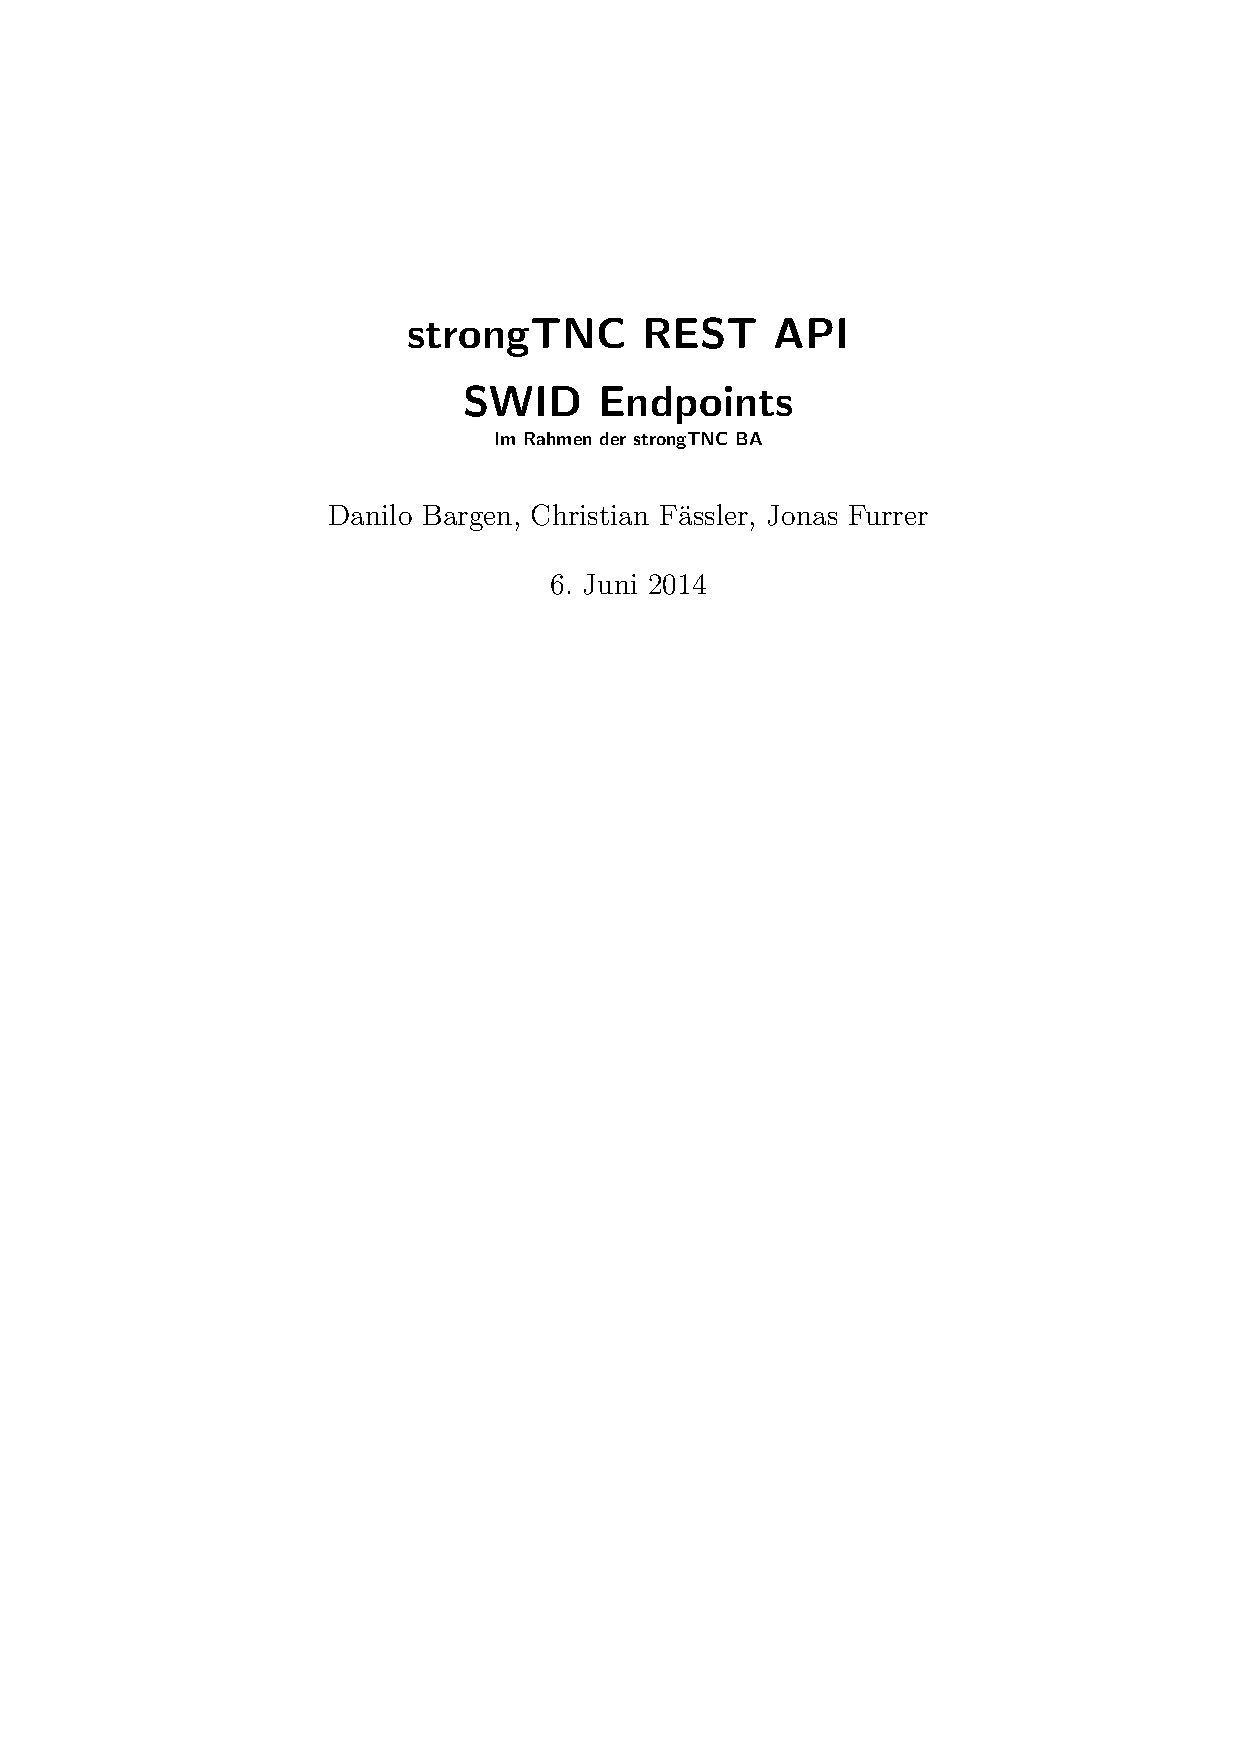
\includepdf[height=\textheight,pages={-},offset=0mm -5mm, frame=true]{other_documents/swid-measurement-manual.pdf}


\section{Eigenständigkeitserklärung}
Wir erklären hiermit, 
\begin{itemize}


\item	dass wir die vorliegende Arbeit selber und ohne fremde Hilfe durchgeführt haben, ausser derjenigen, welche explizit in der Aufgabenstellung erwähnt sind oder mit dem Betreuer schriftlich vereinbart wurden,
\item	dass wir sämtliche verwendeten Quellen erwähnt und gemäss gängigen wissenschaftlichen Zitierregeln korrekt angegeben haben.
\item dass wir keine durch Copyright geschützten Materialien (z.B. Bilder) in dieser Arbeit in unerlaubter Weise genutzt haben. 

\end{itemize}

Rapperswil, 13.06.2014


\begin{tabular}{lll}
	Danilo Bargen & Christian Fässler & Jonas Furrer \\

\includegraphics[scale=0.7]{images/unterschrift-danilo} & 
\includegraphics[scale=0.7]{images/unterschrift-chrigi} & 
\includegraphics[scale=0.7]{images/unterschrift-jonas} \\
\end{tabular} 
